\section{Überblick}

\begin{frame}
  {Überblick}
  \pause
  \begin{itemize}[<+->]
    \item Was sind Wörter?
    \item Lexikalisches vs.\ syntaktisches Wort
      \Halbzeile
    \item Wozu Wortklassen?
    \item \rot{Bedeutungsklassen} und Wortklassen
    \item \alert{Morphologie} von Wortklassen
%    \item \alert{Syntax} von Wortklassen
      \Halbzeile
    \item wichtige Wortklassen
      \begin{itemize}[<+->]
        \item Nomen
        \item Verb
        \item Präposition
        \item Adverb
        \item \ldots
      \end{itemize}
      \Halbzeile
    \item \citet[Kap.~6]{Schaefer2018b} | zusätzlich \citet{Engel2009}
  \end{itemize}
\end{frame}


\section{Wörter}

\begin{frame}
  {Ebenen und Einheiten}
  \pause
  Kombinatorik von Wortbestandteilen und von Wörtern:
  \pause
  \Zeile
  \begin{exe}
    \ex
    \begin{xlist}
      \ex[]{Staat-es}
      \pause
      \ex[*]{Tür-es}
    \end{xlist}
    \pause
    \Zeile
    \ex
    \begin{xlist}
      \ex[]{Der Satz ist eine grammatische Einheit.}
      \pause
      \ex[*]{Die Satz ist eine grammatische Einheit.}
    \end{xlist}
  \end{exe}
\end{frame}

\begin{frame}
  {Alle Wörter haben eine Bedeutung?}
  \pause
  \begin{exe}
    \ex \alert{Es} \alert{wird} schon wieder früh dunkel.
    \pause
    \ex Kristine denkt, \alert{dass} \alert{es} bald regnen \alert{wird}.
    \pause
    \ex Adrianna \alert{hat} gestern \alert{den} Keller inspiziert.
    \pause
    \ex Camilla \alert{und} Emma sehen \alert{sich} \alert{die} Fotos \alert{an}.
  \end{exe}
  \Zeile
  \pause
  \large
  \alert{Bedeutungstragende} Wörter und \alert{Funktionswörter}
\end{frame}

\begin{frame}
  {Morphologie und Syntax}
  \pause
  \begin{itemize}[<+->]
    \item Kombinatorik für \alert{Wortbestandteile}: Morphologie
      \begin{itemize}[<+->]
        \item Wortbestandteile \zB mit \alert{Umlaut}: \textit{rot} -- \textit{röter}
        \item oder \alert{Ablaut}: \textit{heben} -- \textit{hob}
      \end{itemize}
    \item Kombinatorik für \alert{Wörter}: Syntax
      \Zeile
    \item \alert{Zirkuläre oder leere Definitionen?}
    \item \rot{Nein!} Prinzip: eigene Regularität → eigene Struktur
      \Zeile
    \item Wortbestandteile \alert{nicht trennbar}:
      \begin{itemize}
        \item \textit{heb-t}\\
          *\textit{heb mit Mühe t}
        \item \textit{Ge-hob-en-heit} \\
          *\textit{Gehoben anspruchsvolle heit}
        \item \textit{Sie geht schnell heim.}\\
          \textit{Schnell geht sie heim.}
      \end{itemize}
  \end{itemize}
\end{frame}

\begin{frame}
  {Wort und Wortform I}
  \pause
  \begin{exe}
    \ex
    \begin{xlist}
      \ex (der) Tisch
      \pause
      \ex (den) Tisch
      \pause
      \ex (dem) Tisch\alert{e}
      \pause
      \ex (des) Tisch\alert{es}
      \pause
      \ex (die) Tisch\alert{e}
      \pause
      \ex (den) Tisch\alert{en}
    \end{xlist}
  \end{exe}
  \pause
  \begin{exe}
    \ex
    \begin{xlist}
      \ex Der \_\_\_\ ist voll hässlich.
      \pause
      \ex Ich kaufe den \_\_\_ nicht.
      \pause
      \ex Wir speisten am \_\_\_\ des Bundespräsidenten.
      \pause
      \ex Der Preis des \_\_\_\ ist eine Unverschämtheit.
      \pause
      \ex Die \_\_\_\ kosten nur noch die Hälfte.
      \pause
      \ex Mit den \_\_\_\ können wir nichts mehr anfangen.
    \end{xlist}
  \end{exe}
\end{frame}

\begin{frame}
  {Wort und Wortform II}
  \pause
  \begin{block}{Wortform}
    Eine Wortform ist eine in syntaktischen Strukturen auftretende und in diesen Strukturen nicht weiter zu unterteilende Einheit.
    [\ldots]
  \end{block}
  \Zeile
  \pause
  \begin{block}{Lexikalisches Wort}
    Das (\alert{lexikalische}) \alert{Wort} ist eine Repräsentation von paradigmatisch zusammengehörenden Wortformen.
    Für das lexikalische Wort sind die Werte nur für diejenigen Merkmale spezifiziert, die in allen Wortformen des Paradigmas dieselben Werte haben.
    [\ldots]
  \end{block}
\end{frame}

\section{Methode}

\begin{frame}
  {Klassische Grundschul-Wortarten}
  \pause
  \scalebox{0.85}{%
  \begin{minipage}{\textwidth}
    \begin{itemize}[<+->]
      \item Dingwort
      \item Tuwort, Tätigkeitswort
      \item Wiewort, Eigenschaftswort
      \item Umstandswort
      \Halbzeile
      \item Dazu die Vermittlungsversuche:
        \begin{itemize}[<+->]
          \item \alert{Dingwörter} kann man anfassen. \onslide<8->{\rot{D'oh!}}
            \pause
          \item \textit{Die ontologischen Referenten von Substantiven\\
            sind physikalische Objekte.} -- Auch falsch!
            \Halbzeile
          \item \alert{Wiewort}: Wie ist die Kanzlerin? -- Katatonisch.
          \item \alert{Tuwort}: Was macht\slash tut Johanna? -- Laufen.
          \item \alert{Umstandswort}: Wie, wo oder warum schläft Johanna? -- Ruhig.
        \end{itemize}
      \Halbzeile
      \item Wieso auch nicht?
        \begin{itemize}[<+->]
          \item Anfassen? Wolken, Ideen, Steckdosen, Rasierklingen, \dots
          \item *Die Kanzlerin ist ehemalig.
          \item Was macht Johanna? -- Hausaufgaben.
          \item Was tut Johanna? -- *Verlaufen. \slash *Sich verlaufen. \slash *Unterliegen.
          \item *Was macht\slash tut der Yoghurt? -- Verschimmeln.
          \item Wie schläft Johanna? -- *Erstaunlicherweise.
        \end{itemize}
    \end{itemize}
  \end{minipage}
  }
\end{frame}

\begin{frame}
  {Ein paar neue Wortarten nach Bedeutungen I}
  \pause
  \begin{itemize}[<+->]
    \item "`Wie, wo, warum?"' \onslide<3->{--- Warum eigentlich nicht drei Wortarten?}
      \Halbzeile
      \pause
    \item \alert{Bewegungsverben}: \textit{laufen}, \textit{springen}, \textit{fahren}, \dots
    \item \alert{Zustandsverben}: \textit{duften}, \textit{wohnen}, \textit{liegen}, \dots
      \Halbzeile
    \item \alert{Konkreta}: \textit{Haus}, \textit{Buch}, \textit{Blume}, \textit{Stier}, \dots
    \item \alert{Abstrakta}: \textit{Konzept}, \textit{Glaube}, \textit{Wunder}, \textit{Kausalität}, \dots
      \Halbzeile
    \item \alert{Zählsubstantive}: \textit{Kumquat}, \textit{Student*in}, \textit{Mikrobe}, \textit{Kneipe}, \dots
    \item \alert{Stoffsubstantive}: \textit{Wasser}, \textit{Wein}, \textit{Zement}, \textit{Mehl}, \dots
  \end{itemize}
\end{frame}

%\begin{frame}
%  {Ein paar neue Wortarten nach Bedeutungen II}
%  \pause
%  Aber Moment mal\dots\\
%  \pause
%  \Zeile
%  \begin{exe}
%    \ex
%    \begin{xlist}
%      \ex \alert{Wein} kann lecker sein.
%      \ex \alert{Eine Kumquat kann} lecker sein.
%      \ex \alert{Kumquats können} lecker sein.
%    \end{xlist}
%     \pause
%     \ex
%     \begin{xlist}
%       \ex Ein Glas \alert{guter Wein}\slash\alert{guten Weins} kostet 10€.
%       \ex Ein Glas \alert{?gute Kumquats}\slash\alert{guter Kumquats} kostet 4€.
%     \end{xlist}
%     \pause
%     \ex
%     \begin{xlist}
%       \ex Johanna hätte gerne \alert{eine Kumquat}.
%       \ex Johanna hätter gerne \alert{einen Wein}.
%     \end{xlist}
%   \end{exe}
%   \pause
%   \Zeile
%   Es gibt hier durchaus auch \alert{formale} Unterschiede.
% \end{frame}

\begin{frame}
  {Morphologische Klassifikation}
  \pause
  \begin{exe}
    \ex
    \begin{xlist}
      \ex{Ich pfeif\alert{e}.\\
      Du pfeif\alert{st}.\\
      Die Schiedsrichterin pfeif\alert{t}.}
        \pause
        \ex{Ich schlaf\alert{e}.\\
        {Du schl\rot{ä}f\alert{st}.}\\
        Die Schiedsrichterin schl\rot{ä}f\alert{t}.}
    \end{xlist}
        \pause
    \ex
    \begin{xlist}
      \ex{der Berg\\
        des Berg\alert{es}\\
        die Berg\alert{e}}
        \pause
      \ex{der Mensch\\
        des Mensch\alert{en}\\
        die Mensch\alert{en}}
        \pause
      \ex{der Staat\\
        des Staat\alert{es}\\
        die Staat\alert{en}}
    \end{xlist}
  \end{exe}
\end{frame}

\begin{frame}
  {Morphologische Klassifikation}
  \pause
  \begin{center}
    \Large Wörter lassen sich in Kategorien einordnen,\\
    je nachdem \alert{welche Merkmale und Formen sie haben}.
  \end{center}
  \Zeile
  \pause
  \begin{itemize}[<+->]
    \item Verben: \textsc{Numerus}, \textsc{Person}, \textsc{Tempus}, \ldots
    \item Substantive: \textsc{Numerus}, \textsc{Genus}, \textsc{Person}\rot{?}, \ldots
  \end{itemize}
\end{frame}

\begin{frame}
  {Achtung!}
  \pause
  \alert{Änderung der Wortklassenzugehörigkeit} eines Wortes:
  \pause
  \Zeile
  \begin{exe}
    \ex\label{ex:paradigmatischeklassifikation017}\begin{xlist}
      \ex{Wir sind des \alert{Wanderns} müde.}
      \pause
      \ex{Wir \alert{wandern}.}
    \end{xlist}
  \end{exe}
  \pause
  \Zeile
  $\Rightarrow$ \rot{Zwei verschiedene} lexikalische Wörter.
  \pause
  \begin{itemize}[<+->]
    \item \textit{Wandern}: \textsc{Numerus}, \textsc{Genus}, \ldots
    \item \textit{wandern}: \textsc{Numerus}, \textsc{Person}, \textsc{Tempus}, \ldots
  \end{itemize}
\end{frame}


% \begin{frame}
%   {Syntaktische Klassifikation}
%   \pause
%   \begin{exe}
%     \ex
%     \begin{xlist}
%       \ex[]{Alexandra spielt schnell \alert{und} präzise.}
%       \pause
%       \ex[*]{Alexandra spielt schnell \alert{obwohl} präzise.}
%       \pause
%       \ex[]{Alexandra \alert{und} Dzsenifer spielen eine gute Saison.}
%       \pause
%       \ex[*]{Alexandra \alert{obwohl} Dzsenifer spielen eine gute Saison.}
%     \end{xlist}
%     \pause
%     \Zeile
%     \ex
%     \begin{xlist}
%       \ex[]{Alexandra spielt herausragend,\\
%         \alert{obwohl} der Leistungsdruck hoch ist.}
%       \pause
%       \ex[*]{Alexandra spielt herausragend,\\
%         \alert{und} der Leistungsdruck hoch ist.}
%     \end{xlist}
%   \end{exe}
%     \pause
%     \Zeile
%     Alles nur wegen der Bedeutung?
% \end{frame}
% 
% \begin{frame}
%   {Syntaktische Klassifikation}
%   \pause
%   \begin{center}
%     \Large Wörter lassen sich in Kategorien einordnen,\\
%     je nachdem \alert{in welchen syntaktischen Kontexten\\
%     sie auftreten}.
%   \end{center}
%   \Zeile
%   \pause
%   \begin{itemize}[<+->]
%     \item Konjunktionen: zwischen zwei gleichartigen Satzteilen
%     \item Komplementierer: am Anfang bestimmter Nebensätze
%   \end{itemize}
% \end{frame}



\begin{frame}[fragile]
  {Filter}
  \begin{itemize}
    \item<2-> Kapitel 2: \alert{Kategorien} definiert über Merkmale und Werte.
      \begin{itemize}[<+->]
        \item<3-> Hat \textsc{Numerus} oder nicht?
        \item<4-> Hat \textsc{Genus} oder nicht?
        \item<5-> \dots
      \end{itemize}
  \end{itemize}
  \begin{center}
    \scalebox{0.7}{
    \begin{minipage}{\textwidth}  
    \begin{forest}
      /tikz/every node/.append style={font=\footnotesize},
      for tree={l sep=2em, s sep=2.5em},
      [\textit{Wort}, intrme, {visible on=<6->}, for children={visible on=<7->}
        [{Hat  Numerus?}, decide, for children={visible on=<8->}
          [\textit{flektierbar}, intrme, yes, {visible on=<9->}, for children={visible on=<11->}
            [{Ist finit  flektierbar?}, decide, {visible on=<11->}, for children={visible on=<12->}
              [\textbf{Verb}, finall, yes, {visible on=<13->}]
              [\textit{Nomen}, intrme, no, {visible on=<14->}]
            ]
          ]
          [\textit{nicht flektierbar}, intrme, no, {visible on=<10->}, for children={visible on=<15->}
            [{Hat Valenz-\slash  Kasusrektion?}, decide, {visible on=<15->}, for children={visible on=<16->}
              [\textbf{Präposition}, finall, yes, {visible on=<17->}]
              [\textit{andere}, intrme, no, {visible on=<18->}]
            ]
          ]
        ]
      ]
    \end{forest}
   \end{minipage}
   }
  \end{center}
\end{frame}


\section{Einige Wortklassen}

\begin{frame}
  {Flektierbare Wörter: Numerus}
  \pause
  \begin{exe}
    \ex
    \begin{xlist}
      \ex Tüte, Tüten
      \pause
      \ex Baum, Bäume
    \end{xlist}
    \pause
    \ex
    \begin{xlist}
      \ex (ich) gehe, (wir) gehen
      \pause
      \ex (du) gehst, (ihr) geht
    \end{xlist}
    \Zeile
    \pause
    \ex
    \begin{xlist}
      \ex \orongsch<12->{Ein} \orongsch<13->{roter} \alert<8->{Apfel} \rot<9->{hängt} am Baum.
      \pause
      \ex \orongsch<14->{Rote} \alert<10->{Äpfel} \rot<11->{hängen} am Baum.
    \end{xlist}
  \end{exe}
  \Zeile
  \pause
  \pause
  \pause
  \pause
  \pause
  \pause
  \pause
  \pause
  Als \alert{Kongruenzmerkmal} ist Numerus in der Definition\\
  der flektierbaren Wortklassen \alert{strukturell motiviert}.
\end{frame}

\begin{frame}
  {Substantive vs.\ Nomina}
  \pause
  \begin{exe}
    \ex \alert<5->{Die stärkste} \rot<5->{Gewichtheberin} wurde Weltmeisterin.
    \pause
    \ex \alert<5->{Der stärkste} \rot<5->{Versuch} war der zweite.
    \pause
    \ex \alert<5->{Das höchste} \rot<5->{Gewicht} wurde von Tatjana gerissen.
  \end{exe}
  \Zeile
  \pause
  \pause
  \begin{itemize}[<+->]
    \item \rot{Substantive}: festes Genus
    \item \alert{andere Nomina} (Artikel\slash Pronomen, Adjektiv):\\
      Genuskongruenz mit dem Substantiv
  \end{itemize}
\end{frame}

\begin{frame}
  {Adjektive}
  \pause
  \begin{exe}
    \ex
    \begin{xlist}
      \ex Gestern wurde \alert<6->{kein} \rot<3->{großer} \alert<6->{Ball} gespielt.
      \ex Gestern wurde \alert<6->{der} \rot<3->{große} \alert<6->{Ball} gespielt.
    \end{xlist}
    \pause
    \pause
    \ex
    \begin{xlist}
      \ex Gestern wurden \alert<6->{keine} \rot<5->{großen} \alert<6->{Bälle} gespielt.
      \ex Gestern wurden \alert<6->{die} \rot<5->{großen} \alert<6->{Bälle} gespielt.
      \ex Gestern wurden \onslide<6->{\alert{\_}}\ \rot<5->{große} \alert<6->{Bälle} gespielt.
    \end{xlist}
  \end{exe}
  \Zeile
  \pause
  \pause
  \pause
  \centering
  \resizebox{0.4\textwidth}{!}{
    \begin{tabular}{lllllll}
      \toprule
      \multicolumn{3}{l}{} & \textbf{Mask} & \textbf{Neut} & \textbf{Fem} & \textbf{Pl} \\
      \midrule
      \multirow{4}{*}{\textbf{stark}} & \textbf{Nom} & \multirow{4}{*}{heiß-} & er & es & e & e \\
      & \textbf{Akk} && en & es & e & e \\
      & \textbf{Dat} && em & em & er & en \\
      & \textbf{Gen} && en & en & er & er \\
      \midrule
      \multirow{4}{*}{\textbf{schwach}} & \textbf{Nom} & \multirow{4}{*}{(der) heiß-} & e & e & e & en \\
      & \textbf{Akk} && en & e & e & en \\
      & \textbf{Dat} && en & en & en & en \\
      & \textbf{Gen} && en & en & en & en \\
      \midrule
      \multirow{4}{*}{\textbf{gemischt}} & \textbf{Nom} & \multirow{4}{*}{(kein) heiß-} & er \Dim & es \Dim & e & en \\
      & \textbf{Akk} && en & es \Dim & e & en \\
      & \textbf{Dat} && en & en & en & en \\
      & \textbf{Gen} && en & en & en & en \\
      \bottomrule
    \end{tabular}
  }
\end{frame}

% \begin{frame}
%   {Präpositionen flektieren nicht und regieren Kasus}
%   \pause
%   \begin{exe}
%     \ex
%     \begin{xlist}
%       \ex{\alert<3->{Mit} \rot<4->{dem kaputten Rasen} ist nichts mehr anzufangen.}
%       \pause
%       \pause
%       \pause
%       \ex{\alert<6->{Angesichts} \rot<7->{des kaputten Rasens} wurde das Spiel abgesagt.}
%     \end{xlist}
%   \end{exe}
%   \pause
%   \pause
%   \pause
%   \Zeile
%   \begin{block}{Rektion}
%     In einer Rektionsrelation werden durch die regierende Einheit (das \alert{Regens}) Werte für bestimmte Merkmale\slash Werte (und damit ggf.\ auch die Form) beim regierten Element (dem \alert{Rectum}) verlangt.\\
%   \end{block}
%   \Zeile
%   \pause
%   \begin{block}{Präposition}
%     Präpositionen kasusregieren eine obligatorische Nominalphrase.
%   \end{block}
% \end{frame}
% 
% \begin{frame}
%   {Komplementierer}
%   \pause
%   \begin{exe}
%     \ex
%     \begin{xlist}
%       \ex[]{Ich glaube, [\alert<3->{dass} dieser Nebensatz ein Verb \alert<4->{enthält}].}
%       \ex[]{[\alert<6->{Während} die Spielzeit \alert<7->{läuft}], zählt jedes Tor.}
%       \ex[]{Es fällt ihnen schwer [\rot<8->{zu laufen}].}
%       \ex[\rot<11->{*}]{[\alert<9->{Obwohl} kein Tor \alert<10->{fiel}].}
%     \end{xlist}
%   \end{exe}
%   \Zeile
%   \pause
%   \pause
%   \pause
%   \pause
%   \pause
%   \pause
%   \pause
%   \pause
%   \pause
%   \pause
%   \begin{block}{Komplementierer}
%     Komplementierer leiten Nebensätze ein.\\
%     Die Rede von der \textit{unterordnenden Konjunktion} ist ungeschickt.
%   \end{block}
% \end{frame}
% 
% \begin{frame}
%   {Nicht-flektierbare Wörter im "`Vorfeld"'}
%   \pause
%   Was steht im unabhängigen Aussagesatz am Satzanfang?\\
%   \pause
%   {\rot{Antworten Sie nie mehr mit "`das Subjekt"'!}}
%   \pause
%   \begin{exe}
%     \ex\label{ex:adverbenadkopulasundpartikeln038}
%     \begin{xlist}
%       \ex[ ]{\alert<5->{Gestern} hat der FCR Duisburg gewonnen.}
%       \pause
%       \pause
%       \ex[ ]{\alert<7->{Erfreulicherweise} hat der FCR Duisburg gestern gewonnen.}
%       \pause
%       \pause
%       \ex[ ]{\alert<9->{Oben} finden wir andere Beispiele.}
%       \pause
%       \pause
%       \ex[*]{\alert<11->{Doch} ist das aber nicht das Ende der Saison.}
%       \pause
%       \pause
%       \ex[*]{\alert<13->{Und} ist die Saison zuende.}
%       \pause
%       \pause
%     \end{xlist}
%     \ex\label{ex:adverbenadkopulasundpartikeln044} Das ist aber \alert{doch} nicht das Ende der Saison.
%   \end{exe}
%   \pause
%   \Viertelzeile
%   \begin{block}{Adverb}
%     Adverben sind die übriggebliebenen nicht-flektierbaren Wörter, die im Vorfeld stehen können.
%   \end{block}
% \end{frame}


\begin{frame}[fragile]
  {"`Alle Wortklassen"'}
  \pause
  \begin{center}
    \scalebox{0.35}{
    \begin{minipage}{\textwidth}
    \centering
    \begin{forest}
      /tikz/every node/.append style={font=\footnotesize},
      for tree={l sep=2em, s sep=2.5em, align=center},
      [\textit{Wort}, intrme
        [{Hat\\Numerus?}, decide
          [\textit{flektierbar}, intrme, yes
            [{Ist finit\\flektierbar?}, decide
              [\textbf{Verb}, finall, yes]
              [\textit{Nomen}, intrme, no
                [{Hat festes\\Genus?}, decide
                  [\textbf{Substantiv}, finall, yes]
                  [{\textit{anderes}\\\textit{Nomen}}, intrme, no
                    [{Hat Stärke-\\flexion?}, decide
                      [\textbf{Adjektiv}, finall, yes]
                      [{\textit{Artikel\slash}\\\textit{Pronomen}}, intrme, no]
                    ]
                  ]
                ]
              ]
            ]
          ]
          [\textit{nicht flektierbar}, intrme, no
          [{Hat Valenz-\slash\\Kasusrektion?}, decide
              [\textbf{Präposition}, finall, yes]
              [\textit{andere}, intrme, no
                [{Leitet Neben-\\Sätze ein?}, decide
                  [\textbf{Komplementierer}, finall, yes]
                  [{\textit{Partikel\slash}\\\textit{Adverb}}, intrme, no
                    [{Kann das Vor-\\feld besetzen?}, decide
                      [{\textit{Adverb\slash}\\\textit{Adkopula}}, intrme, yes
                        [{Wird typisch mit\\Kopula verwendet?}, decide
                          [\textbf{Adkopula}, finall, yes]
                          [\textbf{Adverb}, finall, no]
                        ]
                      ]
                      [\textit{Partikel}, intrme, no
                        [{Kann Sätze\\ersetzen?}, decide
                          [\textbf{Satzäquivalent}, finall, yes]
                          [\textit{andere}, intrme, no
                            [{Kann Konsti-\\tuenten verbinden?}, decide
                              [\textbf{Konjunktion}, finall, yes]
                              [\textit{Rest}, intrme, no]
                            ]
                          ]
                        ]
                      ]
                    ]
                  ]
                ]
              ]
            ]
          ]
        ]
      ]
    \end{forest}
    \end{minipage}
    }
  \end{center}
\end{frame}


\begin{frame}
  {Wie viele Wortklassen gibt es?}
  \pause
  \begin{itemize}[<+->]
    \item Alle Wörter sind \alert{Wörter}.
    \item Also gibt es \rot{eine Wortklasse}.
      \Zeile
    \item Jedes Wort hat \alert{individuelle Eigenschaften}.
    \item Also gibt es \rot{so viele Wortklassen wie Wörter}.
      \Zeile
    \item Wozu brauchen wir überhaupt Wortklassen?\\
      Wortklassen\dots
      \begin{itemize}[<+->]
        \item \dots sind \alert{das Rüstzeug für Morphologie und Syntax}.
        \item \dots erlauben die Formulierung von \rot{Generalisierungen}.
        \item \dots sind so fein unterteilt, wie es unsere Beschreibung erfordert.
        \item \dots sind \rot{nicht universell}!
        \item \dots sind \alert{Artefakte unserer Theorie bzw.\ Grammatik}.
      \end{itemize}
  \end{itemize}
\end{frame}


\section{Schulaufgaben}

\begin{frame}
  {Ein Beispiel aus \textit{Alles klar!} 7\slash 8}
  Hier soll der Gebrauch von \alert{Adjektiven} geübt werden\ldots
  \begin{center}
    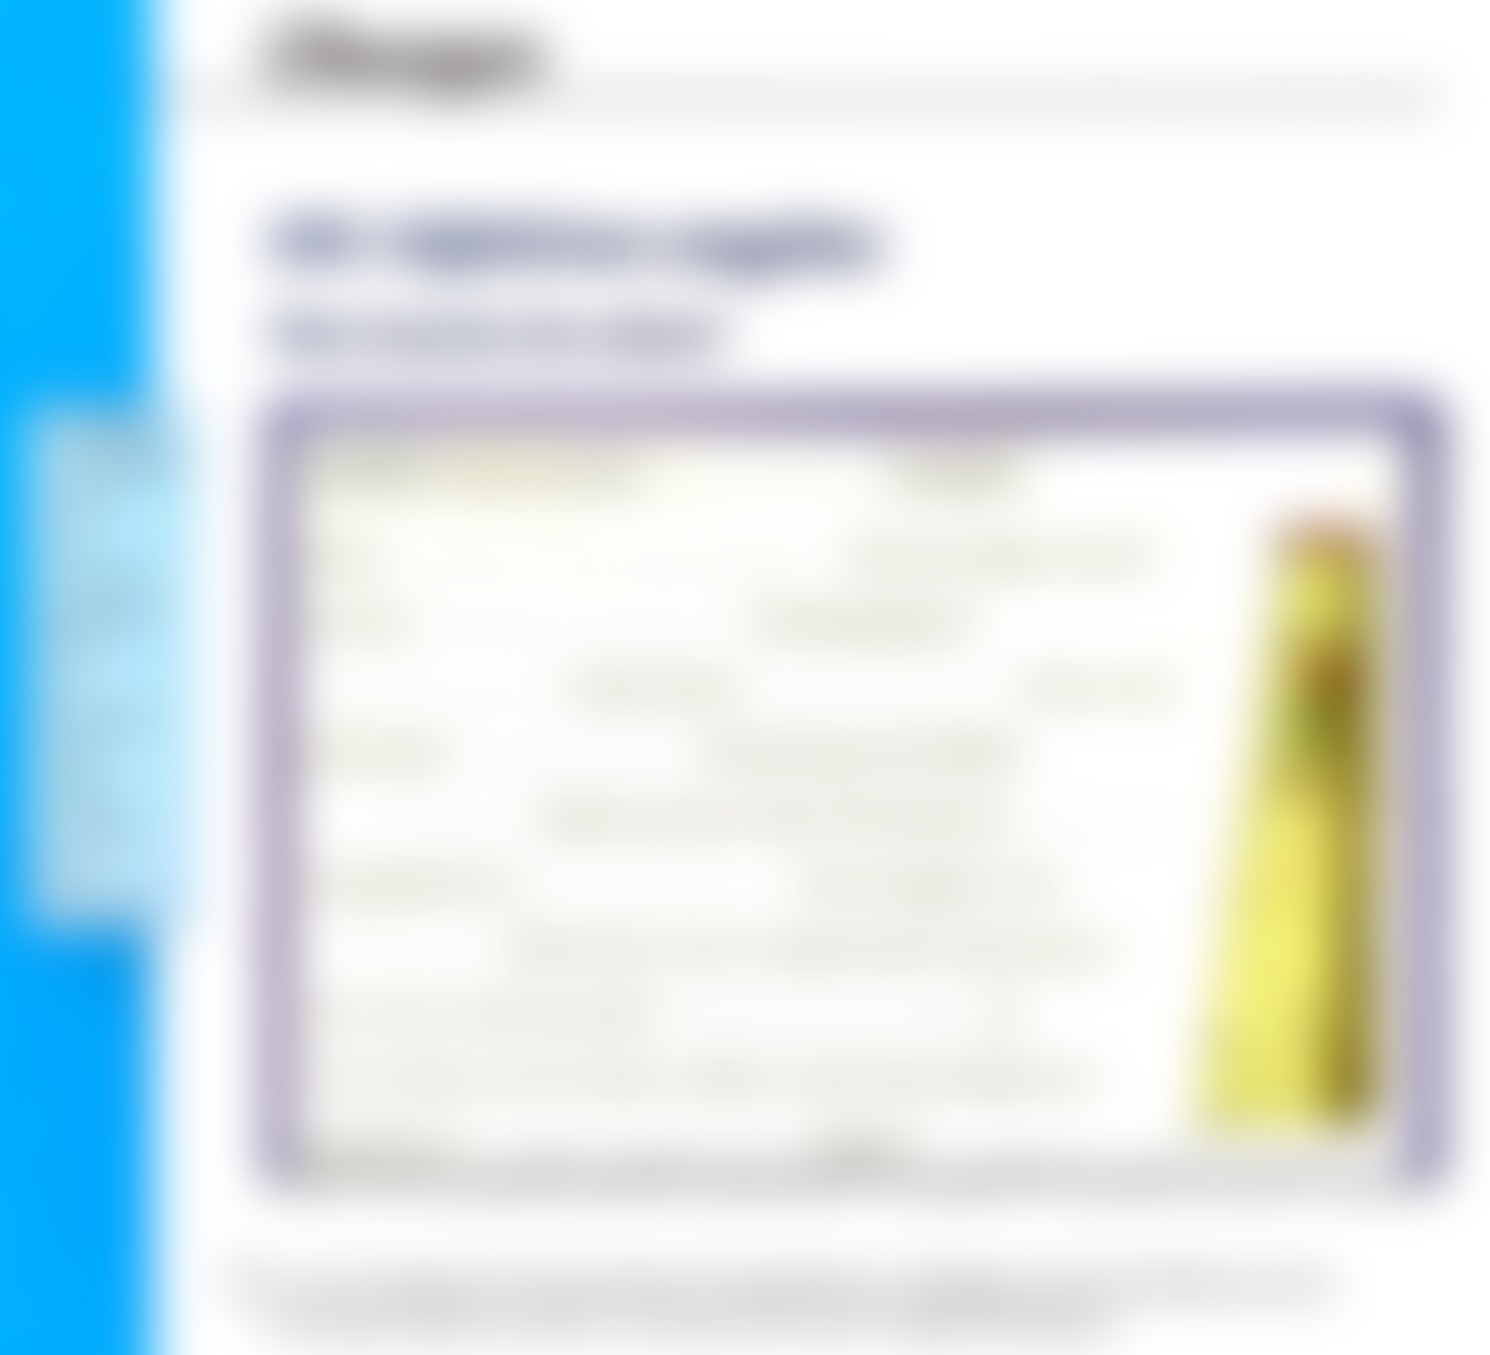
\includegraphics[width=0.5\textwidth]{\GRAPHPATH/adjektive1}
  \end{center}
  \tiny Maempel, Oppenländer \& Scholz. 2012. \textit{Alles klar!} 7\slash 8. Lern- und Übungsheft Grammatik und Zeichensetzung. Berlin: Cornelsen.
\end{frame}


\begin{frame}
  {Ein Beispiel aus \textit{Alles klar!} 7\slash 8}
  Hier soll der Gebrauch von \alert{Adjektiven} geübt werden\ldots
  \begin{center}
    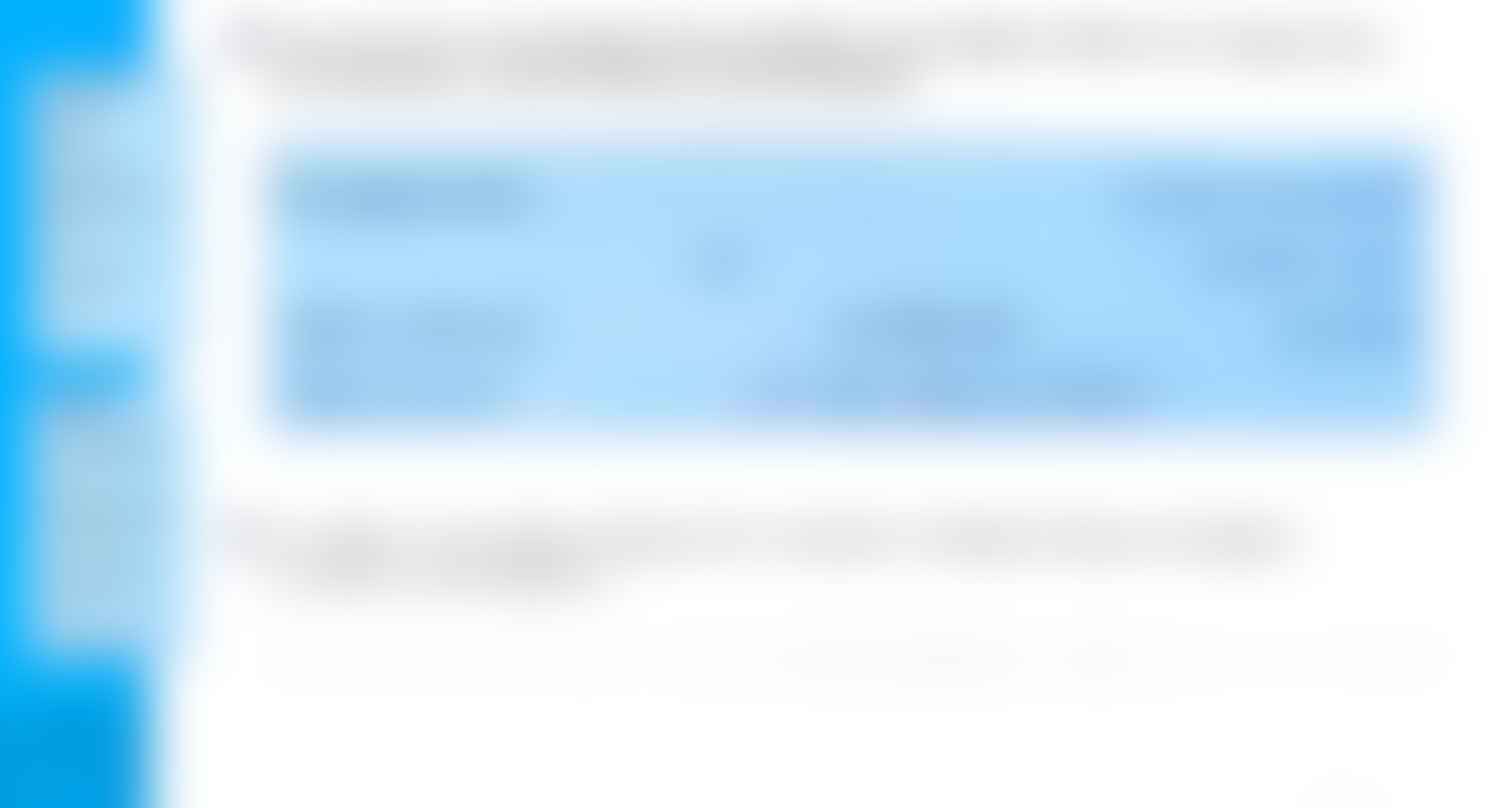
\includegraphics[width=0.6\textwidth]{\GRAPHPATH/adjektive2}
  \end{center}
  \tiny Maempel, Oppenländer \& Scholz. 2012. \textit{Alles klar!} 7\slash 8. Lern- und Übungsheft Grammatik und Zeichensetzung. Berlin: Cornelsen.
\end{frame}


\begin{frame}
  {Warum fehlen hier viele Sorten von Adjektiven?}
  \pause
  \small
  Diese Adjektivklassen fehlen nahezu vollständig in der Aufgabe:
  \pause
  \begin{itemize}[<+->]
    \item \rot{temporal}: der \rot{gestrige} Vorfall
    \item \rot{quantifizierend} (relativ, Zählsubstantiv): \textit{die \rot{zahlreichen} Äpfel}
    \item \rot{quantifizierend} (relativ, Stoffsubstantiv): \textit{\rot{reichlich} Apfelmus}
    \item \rot{quantifizierend} (absolut): \textit{die \rot{drei} Bienen}
    \item \rot{intensional}: \textit{der \rot{ehemalige} Präsident}\slash\textit{die \rot{fiktive} Gestalt}
    \item \rot{phorisch}: \textit{die \rot{obigen}}/\textit{\rot{weiteren}}/\textit{\rot{anderen} Ausführungen}
  \end{itemize}
  \pause
  \Halbzeile
  Fällt Ihnen was auf?
  \pause
  \begin{itemize}[<+->]
    \item Das sind im Wesentlichen die, die \rot{nicht prädikativ verwendbar} sind.
    \item Der Wie-Wort-Test basiert aber auf prädikativer Verwendbarkeit.
    \item Aber viele Adjektive sind nicht prädikativ verwendbar. 
  \end{itemize}
  \pause
  \centering
  \raisebox{0\height}{
\includegraphics[width=3em]{\GRAPHPATH/doh}}
\end{frame}



\section{Übung}

\begin{frame}
  {Wortklassen | Nomina}
  \Zeile
  \centering 
  Suchen Sie im gegebenen Text nach \alert{Nomina},\\
  unterklassifizieren Sie diese und überlegen Sie,\\
  welche Markierungsfunktion ihre Affixe haben.\\
\end{frame}

\section{Vorschau}

\begin{frame}
  {Nächste Woche | Lehn- und Fremdwort}
  \Zeile
  \centering 
  Suchen Sie nach \alert{Definitionen der Begriffe \textit{Lehnwort} und \textit{Fremdwort}}\\
  und finden Sie je fünf \alert{Beispiele} für Lehnwörter, Fremdwörter\\
  (falls Sie abweichende Definitionen für diese beiden Begriffe gefunden haben)\\
  und Wörter, die keins von beidem sind.
\end{frame}
